\chapter{Flow Matching \& SD3}

Un modello generativo ha lo scopo di modellare la distribuzione di probabilità di un insieme di dati. Se abbiamo un dataset con i seguenti dati osservati $\{x^{(1)},x^{(2)},\,\dots\,,x^{(N)}$, l'obbiettivo è quello di imparare una distribuzione in modo tale che:

\begin{equation}
    p_{\operatorname{model}}(x)\approx p_{\operatorname{data}}(x)
\end{equation}

Dove $p_{\operatorname{data}}(x)$ è la distribuzione reale da cui i dati sono stati campionati, a noi sconosciuta, mentre $p_{\operatorname{model}}(x)$ è la distribuzione appresa dal modello generativo. Una volta appresa attraverso un processo trasformativo continuo o discreto, possiamo campionare nuovi dati realistici, simili a quelli presenti nel dataset, calcolare probabilità per stimare quanto è plausibile un nuovo dato, completare dati come riempire le parti mancanti in un'immagine o in una frase, condizionare la generazione su un'informazione generando per esempio una didascalia a partire da un'immagine.

\section{Mappatura diretta e Processi di Markov}
Un primo approccio consiste in una \textbf{mappatura diretta} tramite un modello deterministico $f: \mathbb{R}^d \to \mathbb{R}^d$ tale che $x_1 = f(x_0)$, dove $x_0 \sim p_{\operatorname{data}}(x)$. Tuttavia, per modellare fenomeni complessi, si può optare per un processo continuo nel tempo, come un \textbf{processo di Markov} continuo descritto da una velocità $v_t(x)$ che genera traiettorie di trasformazione tra le due probabilità, ed è proprio quì che entra in gioco il concetto di flusso.

\section{Flusso e Velocità}
Nel contesto dei modelli generativi, il \textbf{flusso} descrive l'evoluzione temporale delle distribuzioni tramite un campo di vettori $v_t(x)$, che rappresenta la velocità con cui un punto nello spazio dei dati si muove al tempo $t$. La dinamica è modellata tramite un'equazione differenziale ordinaria (ODE):
\begin{equation}
    \frac{dx}{dt} = v_t(x), \quad x(0) \sim p_{\operatorname{data}}(x)
\end{equation}

\section{I modelli da cui ci discostiamo}

Affrontiamo in breve i modelli da cui ci discostiamo per poter giungere all'idea del \textbf{Flow Matching} con una base più solida. In primis ci sono i modelli di Stable Diffusion, già approfonditi nel capitolo~\label{chapter15}, essi si basano per la costruzione e la ricostruzione di un'immagine su flussi stocastici, questi flussi sono diversi da quelli citati tramite le equazioni differenziali ordinarie che abbiamo citato prima, seguendo un approccio probabilistico piuttosto che un approccio deterministico. Invece per quanto riguarda quelli che seguono un approccio deterministico in maniera differente da quella citata in precedenza sono i \textbf{Normalizing Flows} e i \textbf{Continuous Normalizing Flows}.

\subsection{Normalizing Flows}

I \textbf{Normalizing Flows} sono una classe di modelli generativi che costruiscono distribuzioni complesse trasformando una distribuzione semplice, come quella gaussiana standard, tramite una serie di trasformazioni invertibili e differenziabili in una più complessa. Partendo da $z \thicksim p_z(z)$, una variabile latente semplice, e $x = f_{\theta}(z)$ la trasformazione appresa, se $f_{\theta}$ è invertibile, la densità $p(x)$ è calcolabile tramite il cambiamento di variabile:

\begin{equation}
    \log p(x) = \log p_z(f_\theta^{-1}(x)) + \log \left|\det\left(\frac{\partial f_\theta^{-1}(x)}{\partial x}\right)\right|
\end{equation}

Il problema più evidente è che il determinante jacobiano può risultare costoso da calcolare e limitare la scelta dell'architettura.

\subsection{Continuous Normalizing Flows}

Per far fronte alla difficolta di calcolo del determinante jacobiano, entra in gioco i \textbf{CNFs} (Continuous Normalizing Flows), essi modellano le trasformazioni in modo continuo nel tempo, tramite un'equazione differenziale ordinaria (ODE), e riscrivono la trasformazione come il flusso di un campo vettoriale appreso.%Fonte: Chen et al., "Neural Ordinary Differential Equations", NeurIPS 2018

\section{Flow Matching}

Il \textbf{Flow Matching} (FM) %(Lipman et al.)
propone un approccio alternativo rispetto a modelli basati su simulazioni costose, che portassero a massimizzare la likelihood come succede nelle CNF, invece di simulare forward o reverse paths, si definisce un percorso probabilistico desiderato tra $\pi_0$ e $\pi_1$, e si cerca di far combaciare il campo di vettori appreso con quello che realizza quel percorso, tra punti reali e punti latenti.

\subsection{Costruzione da Flussi Condizionati}
Un'idea potente è costruire flussi marginali a partire da flussi condizionati, ossia descrivere come una particella passa da $x_0$ a $x_1$ lungo un percorso determinato da una distribuzione $\psi_t(x | x_0, x_1)$.

\subsection{Loss di Flow Matching}
La \textbf{Flow Matching Loss} si basa sulla distanza tra la velocità target $v_t$ la quale descrive come un punto dovrebbe muoversi lungo la traiettoria tra due distribuzioni (nota a partire da $\psi_t$) e quella predetta dal modello $\hat{v}_t$:
\begin{equation}
    \mathcal{L}_{FM} = \mathbb{E}_{x_0,x_1,t} \left[ \left\| \hat{v}_t(\gamma_t) - v_t(\gamma_t) \right\|^2 \right]
\end{equation}

L'uso del punto $\gamma_t$ è legato al fatto che stiamo risolvendo un'equazione differenziale ordinaria (ODE) e desideriamo un punto rappresentativo della traiettoria. In particolare, quando si usa un metodo numerico come il Midpoint Integrator (punto medio), l'approssimazione dell'integrale è più accurata rispetto all'uso diretto degli estremi $x_0$ e $x_1$. Quindi, il training avviene in spazi interpolati per massimizzare la stabilità numerica e l'efficienza del flusso.

\subsection{Marginalization Trick}

L’obiettivo del Marginalization Trick è evitare di campionare intere traiettorie e calcolare comunque le velocità target in modo efficiente. Invece di definire una loss sulla traiettoria completa tra $x_0$ e $x_1$, si considera la distribuzione condizionata $\psi_t(x | x_0, x_1)$, che definisce la probabilità di essere in un certo punto $x$ lungo il percorso. Marginalizzando infine come segue su $x_0, x_1$, campionando il valore $\gamma_t$ solo dopo che sono stati individuati gli endpoint. Questo approccio consente un calcolo efficiente dei target di velocità senza dover simulare interamente le traiettorie.

\begin{equation}
    \mathcal{L}_{FM} =\mathbb{E}_{x_0,x_1}\left[\mathbb{E}_t\left[\mathbb{E}_{\gamma_t\sim\psi_t(\cdot|x_0,x_1)}\|f_\theta(\gamma_t,t) - v_t(\gamma_t|x_0,x_1)\|^2\right]\right]
\end{equation}
È doveroso specificare come la velocità presente nella formula è la velocità condizionata, grazie a questo trucco otteniamo dei vantaggi notevoli, inanzitutto il più importante è che non serve più calcolare le traiettorie intere, rendendo l'addestramento più efficiente e parametrizzabile anche grazie alla possibilità di campionare direttamente $\gamma_t$ da distribuzioni costruite, giungendo al calcolo di una funzione di costo puntuale, sfruttando la distribuzione ponte $\psi_t$ e la velocità condizionata $v_t$.

\subsection{Percorsi Affini e Gaussiani}
Il parametro $\gamma$ può essere calcolato anche tramite degli studi differenti, tramite l'utilizzo dei percorsi affini o di quelli gaussiani:

\subsubsection{Percorso affine}
Sono le traiettorie lineari definite come:
\begin{equation}
    \gamma_t = (1-t)\,x_0 + t\,x_1
\end{equation}
Sono semplici da calcolare, permettono l’uso di una velocità costante $x_1-x_0$, e sono perfetti per il training supervisionato di un flusso deterministico.

\subsubsection{Percorso Gaussiano}
Si basano su interpolazioni tra $x_0$ e $x_1$ che includono un termine di rumore:

\begin{equation}
    \gamma_t = (1-t)\,x_0 + t\,x_1 + \sqrt{t\,(1-t)}\cdot\epsilon, \qquad \epsilon\sim\mathcal{N}(0,I)
\end{equation}

Questo permette di esplorare traiettorie più robuste, simili ai cammini percorsi nei modelli di diffusione, migliorando la copertura dello spazio.

\subsection{Metodologia di Addestramento}
Ci sono ben tre tipologie di addestramento per il Flow Matching, le quali sono descritte in breve quì di seguito
\begin{itemize}
    \item \textbf{Simulation-Free}: il flusso è definito direttamente tramite la specifica del percorso di probabilità e ottimizzando il campo vettoriale di conseguenza, evitando delle simulazioni costose;
    \item \textbf{Gradient-Based}: ottimizzazione con discesa del gradiente per ottimizzare i parametri;
    \item \textbf{Conditional Flow Matching}: il flow matching definisce una funzione obbiettivo chiamata; \textbf{Conditional Flow Matching Objective}, la quale garantisce stime prive di bias dei gradienti e un efficiente allenamento.
\end{itemize}

Come abbiamo potuto vedere solitamente ci troviamo in una situazione in cui abbiamo due distribuzioni: una inziale e una target. Ovviamente per giungere da una all'altra ci saranno delle fasi intermedie, e vi è una procedura di training che viene adottata. Inizialmente si prendono in considerazione in maniera casuale coppie di punti rispettivamente uno della distribuzione inziale e uno della distribuzione target (sì, lo stiamo facendo veramente in maniera casuale), e muoviamo questi punti lungo una traiettoria rettilinea a una velocità costante, questa cosa è visualizzabile in Figura~\ref{fig:FMTrain}.
\begin{figure}
    \centering
    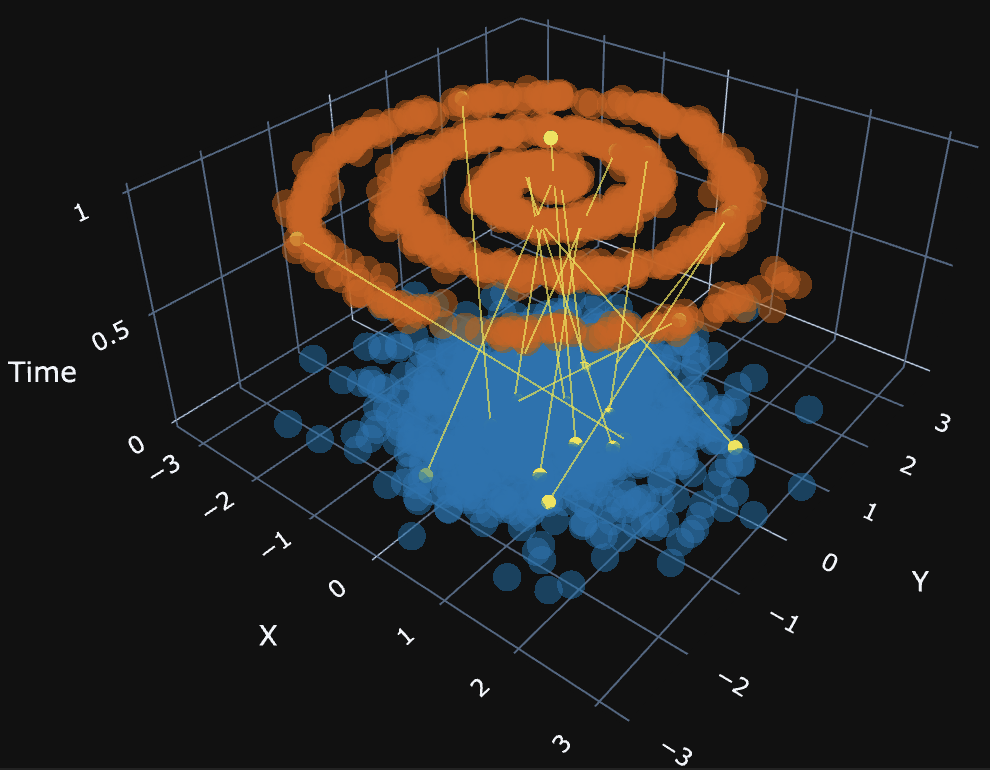
\includegraphics[width=0.7\textwidth]{figure/FMTrain.png}
    \caption{Visualizzazione 3D della procedura di Training, in blu la distribuzione iniziale dei datapoint, in arancione la distribuzione target.}
    \label{fig:FMTrain}
\end{figure}
Ci sono grossi problemi nel far ciò, infatti l'accoppiamento casuale produce molte traiettorie che si incrociano che sono un problema, tuttavia, permetteremo alle traiettorie dei singoli punti di incrociarsi durante l'addestramento del modello. Questo risulta "confuso" per il modello, il quale cercherà di apprendere un campo di velocità, non definito dove le traiettorie si incrociano. Alla fine, però, il modello imparerà a stimare il moto aggregato di molte particelle, che farà la media per arrivare al "moto di massa" del flusso, dando origine a linee di flusso che non si incrociano. Questo è il motivo per cui la corrispondenza dei flussi riguarda la trasformazione delle distribuzioni, non dei singoli punti. Il campo di velocità appreso potrebbe non corrispondere esattamente a nessuna delle nostre traiettorie di addestramento, ma in grado di catturare il flusso statistico necessario per trasformare una distribuzione in un'altra. L'obiettivo dei sistemi di Machine Learning è il seguente: per qualsiasi punto nello spazio e qualsiasi tempo $t$ compreso tra 0 e 1, vogliamo imparare la velocità corretta (direzione e velocità) con cui quel punto dovrebbe muoversi. È come imparare la "mappa del vento" che porterà la nuvola di distribuzione di partenza alla forma della nuvola di distribuzione di destinazione. Poiché le reti neurali sono motori molto utili per l'approssimazione e l'interpolazione, lasceremo che una rete neurale impari a stimare la mappatura tra luoghi e tempi (come input) e velocità (come output).

\begin{python}[frame=trBL]
import torch.nn as nn
import torch.nn.functional as F

class VelocityNet(nn.Module):
    def __init__(self, input_dim, h_dim=64):
        super().__init__()
        self.fc_in  = nn.Linear(input_dim + 1, h_dim)
        self.fc2    = nn.Linear(h_dim, h_dim)
        self.fc3    = nn.Linear(h_dim, h_dim)
        self.fc_out = nn.Linear(h_dim, input_dim)
    
    def forward(self, x, t, act=F.gelu):
        t = t.expand(x.size(0), 1)  
        # Ensure t has the correct dimensions
        x = torch.cat([x, t], dim=1)
        x = act(self.fc_in(x))
        x = act(self.fc2(x))
        x = act(self.fc3(x))
        return self.fc_out(x)

# Instantiate the model
input_dim = 2
model = VelocityNet(input_dim)
\end{python}


Come possiamo vedere questa semplice rete neurale ci permette di ottenere quanto da noi desiderato, ossia la velocità, ma ovviament il software complessivo sfrutterà questa velocità per muovere i punti in giro, e viene utilizzata in equazioni differenziali per descrivere il percorso effettuato con il passare del tempo. La parte più complessa del Flow Matching è la maniera attraverso la quale alleniamo questa rete, per ogni training step dobbiamo seguire i seguenti step:

\begin{enumerate}
    \item Campionare punti casuali dalle distribuzioni di origine e di destinazione e accoppiare i punti;
    \item Campionare tempi casuali compresi tra 0 e 1;
    \item  Calcolare le posizioni in cui questi punti si troverebbero in quei momenti se si muovessero a velocità costante dalla sorgente al bersaglio;
    \item Calcolare la velocità che avrebbero in quei punti se si muovessero a velocità costante, questa cosa viene effettuata dalla rete neurale, per tanto dovrà scoprire da se la velocità costante;
    \item Addestrare la rete a prevedere queste velocità, che finiranno per "cercare la media" quando la rete dovrà fare lo stesso per molti, molti punti.
\end{enumerate}

\begin{figure}
    \centering
    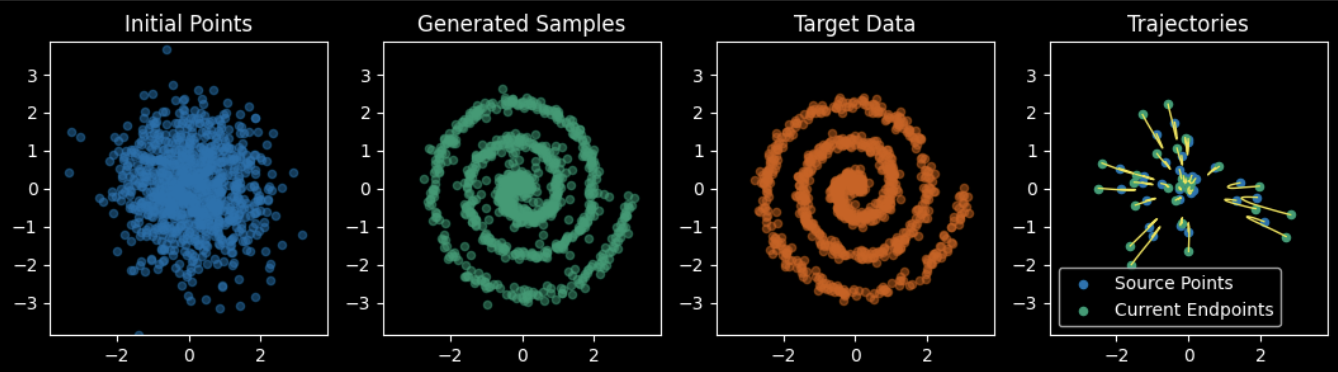
\includegraphics[width=0.9\textwidth]{figure/TrajFM}
    \caption{Rappresentazione di ciò che accade dopo il training alle traiettorie che seguiranno i punti fino a giungere alla distribuzione target.}
    \label{fig:trajFM}
\end{figure}

Anche se le traiettorie risultino essere lisce e non incrociate, la loro curvatura significa che dobbiamo integrare lentamente e con attenzione per evitare di accumulare errori significativi. Ci sono stati dei paper i quali anno approfondito questo dettaglio~\cite{lipman2023flow}, offrendo un modo efficace per accelerare l'integrazione "raddrizzando" le traiettorie curve, attraverso un metodo che chiamano \textbf{Reflow}.

\subsection{Reflow}
Il \textbf{Reflow} è un processo iterativo per migliorare il flusso appreso. Una volta addestrato un modello di velcoità, possiamo utilizzarlo per definire nuovi percorsi, migliorando la qualità delle traiettorie. L'idea del Reflow è che, invece di accoppiare casualmente i punti di origine e di destinazione quando si scelgono le traiettorie rettilinee, si utilizzano "punti di destinazione simulati" integrando i punti di origine in avanti utilizzando il modello di flusso appreso. Quindi utilizziamo questi punti finali come target e assumiamo un movimento lineare come prima (Figura~\ref{fig:reflow}).
\begin{figure}
    \centering
    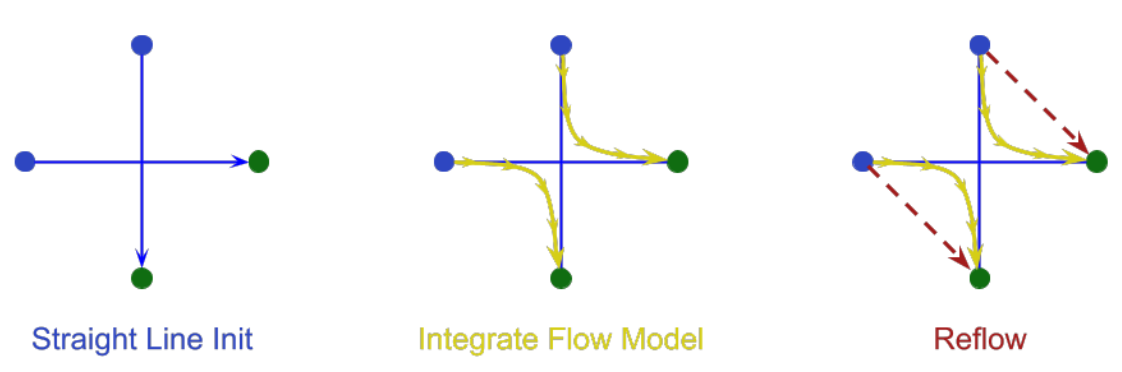
\includegraphics[width=0.8\textwidth]{figure/Reflow}
    \caption{Idea alla base del Reflow, per la considerazione del raggiungimento ai punti target.}
    \label{fig:reflow}
\end{figure}
Ci sono numerose animazioni le quali mettono in luce come sia diretto, ma soprattuto le traiettorie con l'utilizzo del Reflow, siano molto più lineari rispetto a quelle prive di esso, inoltre il passaggio dalle configurazioni iniziali a quelle finali nel Flow Matching, subiscono una sorta di aggregamento iniziale prima di giungere nella posizione finale, cosa che non succede con il Reflow, le quali vanno direttamente nella posizione finale dei valori target.

\subsection{Condizionamento nei Modelli Generativi}
In scenari controllati, si desidera che il modello generi output coerenti con un certo input. Questo si ottiene introducendo \textbf{condizionamenti} nella funzione di costo o nella dinamica del modello, utilizzando la \textbf{Guidance}, essa è un meccanismo che modifica il processo di generazione per ottenere campioni che appartengano a una distribuzione condizionata $p(x|y)$, anche quando il modello è stato addestrato sulla distribuzione marginale $p(x)$ non condizionata. Supponiamo di avere un generatore molto bravo a generare immagini relaistiche di cani, modellando bene  $p(x)$, ma vogliamo generare solo Husky identificati come $y$ (Figura~\ref{fig:Guidance}), dunque voglio proprio una $p(x|y)$, in questi casi la \textbf{Guidance} ci permette di "spingere" la generazione verso i campioni che hanno un'alta probabilità condizionata da noi desiderata, senza dover riaddestrare la rete da zero, ci sono due tipologie principali di Guidance, la \textit{Classifier Guidance} e la \textit{Classifier-Free Guidance}.

\begin{figure}
    \centering
    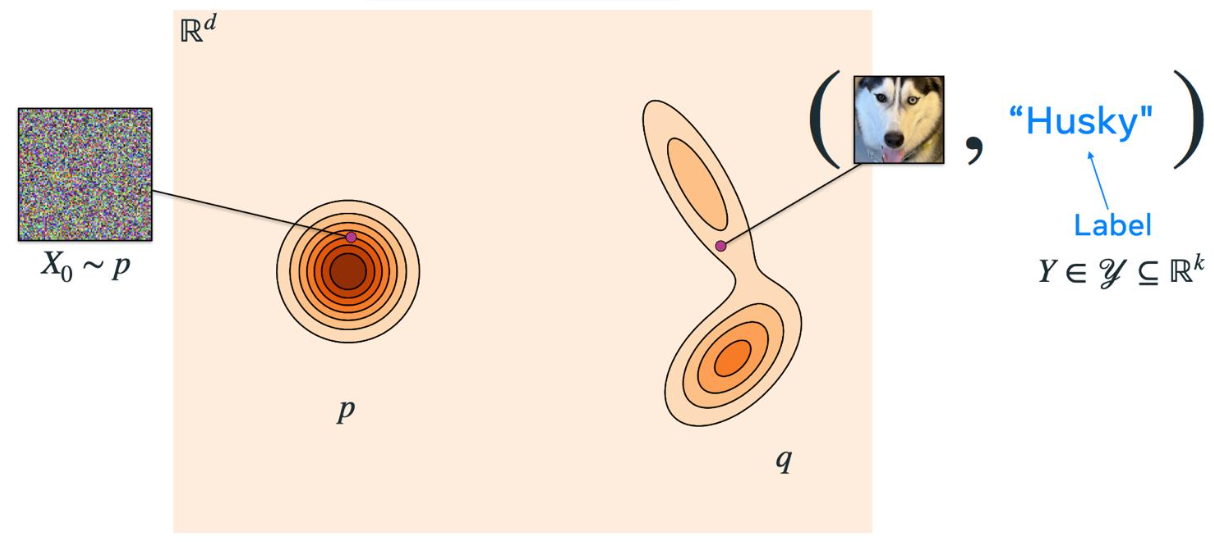
\includegraphics[width=0.7\textwidth]{figure/Guidance}
    \caption{Rappresentazione della Guidance, avendo un modello il quale ci restituisce immagini realistiche di cani, ma vogliamo forzare che ci dia come esito foto di Husky.}
    \label{fig:Guidance}
\end{figure}

\subsubsection{Classifier Guidance}
Questa tecnica utilizza un classificatore pre-addestrato $p_\eta(y\,|\,x)$ per modificare la dinamica:

\begin{equation}
    \nabla_x\log p(x\,|\,y) = \nabla_x\log p(x) + \nabla_x \log p_\eta (y\,|\,x)
\end{equation}

Il generatore segue la discesa del gradiente log-probabilistica detta anche score della distribuzione non condizionata, ma in più segue anche il gradiente di un classificatore, il quale se pensa che l'immagine sia simile a un Husky, la spinge in quella direzione.

\subsubsection{Classifier-Free Guidance}
Questa tecnica invece allena sia il modello condizionato $p(x\,|\,y)$ che quello non condizionato $p(x)$, e si effettua una fusione dei due:

\begin{equation}
    \nabla_x\log \hat{p}(x\,|\,y) = (1 - w)\nabla_x\log p(x) + w\,\nabla_x \log p (y\,|\,x)
\end{equation}
In questo caso non serve un classificatore separato è risulta spesso essere più stabile e più efficace, il peso $w$ controlla quanto fortemente guidare la generazione verso l'obbiettivo desiderato.

\subsubsection{Guidance nel Flow Matching}
Nel Flow Matching invece dei gradienti log-probabilistici detti anche score, si lavora con campi di velocità $u_t(x)$ avendo variazioni sia per quella con classificatore che per quella senza classificatore come visibile di seguito:
\begin{equation*}
    \hat{u}_t(x\,|\,y) = u_t(x) + w\,b_t\nabla_x \log p_\eta(y\,|\,x)
\end{equation*}
\begin{equation*}
    \hat{u}_t(x\,|\,y) =(1-w)\,u_t(x) + w\,u_t(x\,|\,y)
\end{equation*}

\section{T5}

\textbf{T5} sta per \textbf{Text-To-Text Transfer Transformer}, ed è un modello sviluppato da Google Research nel 2020~\cite{raffel2020t5}, il suo concetto chiave è molto semplice, ma potente, ossia quello che tutti i compiti di \textit{Natural Language Processing}, sono formulati come trasformazioni di testo in testo.

\begin{table}[htbp]
\centering
\begin{adjustbox}{width=\textwidth}
\begin{tabular}{|l|p{7cm}|l|}
\hline
\textbf{Task} & \textbf{Input} & \textbf{Output} \\
\hline
Traduzione & \texttt{translate English to German: How are you?} & \texttt{Wie geht es dir?} \\
\hline
Riassunto & \texttt{summarize: The book was about...} & \texttt{It was a book about...} \\
\hline
Classificazione & \texttt{classify sentiment: I love this movie!} & \texttt{positive} \\
\hline
Domanda-Risposta & \texttt{question: What is the capital of France? context: France is a country\dots} & \texttt{Paris} \\
\hline
\end{tabular}
\end{adjustbox}
\caption{Esempi di task gestiti da T5 con input testuali specifici, quì tutto è testo in input, e tutto è testo in output.}
\end{table}
T5 usa una classica architettura Transformer encoder-decoder, simile a quella dei modelli di traduzione neurale~\cite{vaswani2017attention}, l'encoder legge l'input testuale e lo rappresenta come sequenza di vettori, mentre il decoder genera l'output testuale token per token, usando l'attenzione sui vettori prodotti dall'encoder, dunque è diverso da BERT e GPT come abbiamo visto nel capitolo~\ref{cap:14}.

\subsection{Masked Attention}
T5 utilizza la \textbf{Masked Attention}, nella self-attention classica, ogni token può guardare tutti gli altri token della sequenza, ma in questo caso i token, non possono guardare in avanti nella sequenza, nel decoder stai generando un testo token per token e durante l'addestramento hai già tutto l'output target a disposizione, ma devi impedire che il modello "bari" guardando i token futuri.

\subsection{Obbiettivi di Training}

T5 non è addestrato su una next-token prediction o masked token prediction standard, invece è addestrato sulla \textbf{Span Corruption}, la quale rimuove casualmente degli span (frammenti di testo) da l testo, l'input diventa il testo con span mascherati, l'output invece saranno gli span rimossi, permettendo al modello di imparare a ricostruire il testo. La forza di T5 è anche quella di essere stato allenato su uno dei dataset più puliti e grandi disponibili al momento chiamato C4 Dataset (Colossal Clean Crawled Corpus), inoltre dopo il pre-training viene effettuato un fine-tuning su dei task specifici come la traduzione, il raissunto, ecc\dots

\section{DiT}
\textbf{DiT} è un \textbf{Vision Transformer}~\cite{dosovitskiy2021vit}, i quali trattano un'immagine come una sequenza di patch (piccoli blocchi dell'immagine) e la elaborano come se fosse una frase, usando il transformer (Figura~\ref{fig:ViT}). DiT tuttavia è addestrato sui documenti come immagini~\cite{li2023dit}, progettato per comprendere la struttura e il contenuto visivo di documenti senza testo esplicito.
\begin{figure}
    \centering
    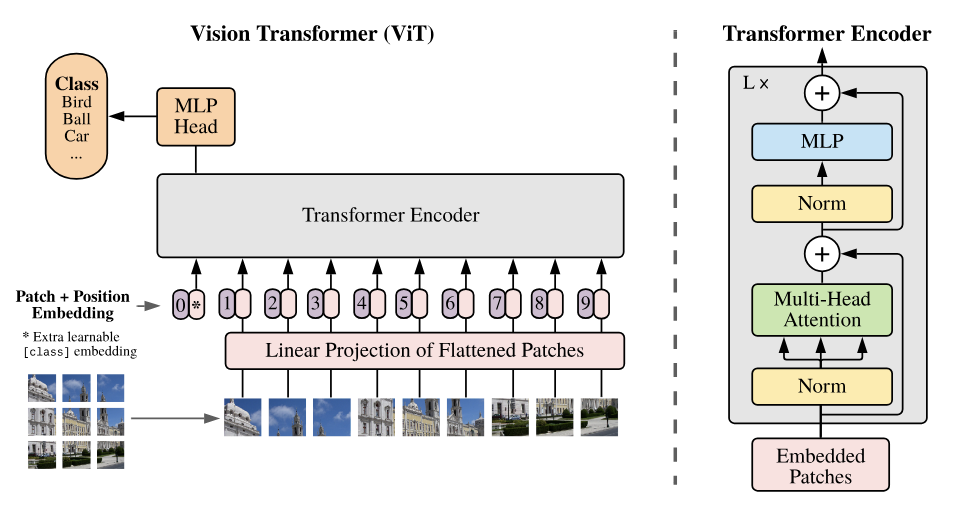
\includegraphics[width=0.7\textwidth]{figure/VisionTransformer}
    \caption{Panoramica del modello. Dividiamo un'immagine in patch di dimensioni fisse, incorporiamo linearmente ciascuna di esse, aggiungiamo le incorporazioni di posizione e diamo la sequenza di vettori risultante a un codificatore Transformer standard. Per eseguire la classificazione, utilizziamo l'approccio standard che prevede l'aggiunta di un "token di classificazione" apprendibile alla sequenza.}
    \label{fig:ViT}
\end{figure}
DiT utilizza la stessa struttura dei Vision Transformer, l'immagine del documento viene divisa in patch, e ognuno di questi patch diventa un embedding, gli embedding vengono processati da stack di Transformer encoder, e come nel ViT, c'è un [CLS] token il cui embedding finale può essere usato per classificazione o altre task globali. DiT è pre-addestrato su documenti, seguendo task come la classificazione dei documenti, la rilevazione del layout e delle tabelle.
\section{MMDiT}

\textbf{MMDiT} è un'estensione di DiT che integra testo e immagine in un unico framework Transformer~\cite{zhang2023mmdetdit}, è pensato per task multimodali, come la comprensione congiunta del layout e del contenuto testuale, mentre DiT lavora solamente sull'immagine, esso lavora su immagine + testo.

\begin{table}[htbp]
\centering
\begin{adjustbox}{width=\textwidth}
\begin{tabular}{|l|p{5.5cm}|p{6cm}|}
\hline
\textbf{Caratteristica} & \textbf{DiT} & \textbf{MMDiT} \\
\hline
Modalità input & Solo immagine & Immagine + Testo \\
\hline
Architettura base & Vision Transformer & Multimodal Transformer (visivo + testuale) \\
\hline
Positional embedding & 2D patches & 2D patches + 2D bounding box \\
\hline
Addestramento & Supervised / Self-supervised & Multimodal supervision \\
\hline
Vantaggi & No OCR necessario & Più preciso nei task semantici \\
\hline
Task principali & Layout, classificazione & VQA, estrazione, analisi semantica \\
\hline
\end{tabular}
\end{adjustbox}
\caption{Confronto tra DiT e MMDiT per la comprensione dei documenti.}
\end{table}

\section{SD3}

\textbf{SD3} invece è un modello di generazione condizionata di immagini basato sull'architettura dei modelli di diffusione~\cite{stablediffusion3}, e rappresenta una delle più recenti evoluzioni di stable diffusion, ottimizzato per qualità, scalabilità e flessibilità d'uso in vari contesti multimodali, \textbf{SD3} (Stable Diffusion 3) è la terza generazione del modello \textit{Stable Diffusion}, rilasciata da Stability AI. È stato progettato per superare i limiti delle versioni precedenti, con un focus particolare sulla coerenza testuale, l'alta risoluzione, multi-condizionalità e la scalabilità. A differenza dei precedenti modelli, SD3 non è un puro modello di diffusione tradizionale, ma è influenzato dal paradigma \textbf{Flow Matching}, il che significa che impara una mappa deterministica dello spazio latente e l'immagine target, ispirandosi alla teoria del flusso. La grande forza è anche che esso utilizza T5 come modello di testo, creando la sua architettura come un'architettura a blocchi.
\vspace{0.8cm}
\begin{figure}[htbp]
    \centering
    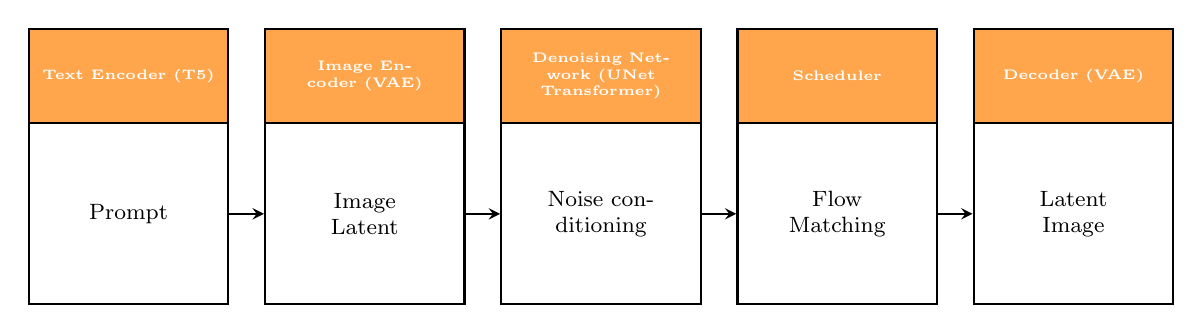
\begin{tikzpicture}[
    % Definizione degli stili
    main_block/.style={
        rectangle,
        draw=black,
        thick,
        minimum width=2.5cm,
        minimum height=3.5cm,
        fill=white
    },
    header/.style={
        rectangle,
        draw=black,
        thick,
        minimum width=2.5cm,
        minimum height=1.2cm,
        fill=orange!70,
        text=white,
        font=\tiny\bfseries,
        align=center,
        text width=2.3cm
    },
    content/.style={
        rectangle,
        draw=black,
        thick,
        minimum width=2.5cm,
        minimum height=2.3cm,
        fill=white,
        font=\footnotesize,
        align=center,
        text width=2.3cm
    },
    arrow/.style={
        ->,
        thick,
        >=stealth
    }
]

% Posizioni dei blocchi
\coordinate (pos1) at (0, 0);
\coordinate (pos2) at (3, 0);
\coordinate (pos3) at (6, 0);
\coordinate (pos4) at (9, 0);
\coordinate (pos5) at (12, 0);

% Blocco 1: Text Encoder
\node[header] (h1) at (pos1) {Text Encoder (T5)};
\node[content] (c1) at ([yshift=-1.75cm]pos1) {Prompt};

% Blocco 2: Image Encoder
\node[header] (h2) at (pos2) {Image Encoder (VAE)};
\node[content] (c2) at ([yshift=-1.75cm]pos2) {Image\\Latent};

% Blocco 3: Denoising Network
\node[header] (h3) at (pos3) {Denoising Network (UNet Transformer)};
\node[content] (c3) at ([yshift=-1.75cm]pos3) {Noise conditioning};

% Blocco 4: Scheduler
\node[header] (h4) at (pos4) {Scheduler};
\node[content] (c4) at ([yshift=-1.75cm]pos4) {Flow\\Matching};

% Blocco 5: Decoder
\node[header] (h5) at (pos5) {Decoder (VAE)};
\node[content] (c5) at ([yshift=-1.75cm]pos5) {Latent\\Image};

% Frecce tra i blocchi (verso destra)
\draw[arrow] (c1.east) -- (c2.west);
\draw[arrow] (c2.east) -- (c3.west);
\draw[arrow] (c3.east) -- (c4.west);
\draw[arrow] (c4.east) -- (c5.west);

\end{tikzpicture}
    \caption{Schema della pipeline del modello di Stable Diffusion 3.}
\end{figure}

